% Options for packages loaded elsewhere
\PassOptionsToPackage{unicode}{hyperref}
\PassOptionsToPackage{hyphens}{url}
\PassOptionsToPackage{dvipsnames,svgnames,x11names}{xcolor}
%
\documentclass[
  letterpaper,
  DIV=11,
  numbers=noendperiod]{scrartcl}

\usepackage{amsmath,amssymb}
\usepackage{iftex}
\ifPDFTeX
  \usepackage[T1]{fontenc}
  \usepackage[utf8]{inputenc}
  \usepackage{textcomp} % provide euro and other symbols
\else % if luatex or xetex
  \usepackage{unicode-math}
  \defaultfontfeatures{Scale=MatchLowercase}
  \defaultfontfeatures[\rmfamily]{Ligatures=TeX,Scale=1}
\fi
\usepackage{lmodern}
\ifPDFTeX\else  
    % xetex/luatex font selection
\fi
% Use upquote if available, for straight quotes in verbatim environments
\IfFileExists{upquote.sty}{\usepackage{upquote}}{}
\IfFileExists{microtype.sty}{% use microtype if available
  \usepackage[]{microtype}
  \UseMicrotypeSet[protrusion]{basicmath} % disable protrusion for tt fonts
}{}
\makeatletter
\@ifundefined{KOMAClassName}{% if non-KOMA class
  \IfFileExists{parskip.sty}{%
    \usepackage{parskip}
  }{% else
    \setlength{\parindent}{0pt}
    \setlength{\parskip}{6pt plus 2pt minus 1pt}}
}{% if KOMA class
  \KOMAoptions{parskip=half}}
\makeatother
\usepackage{xcolor}
\setlength{\emergencystretch}{3em} % prevent overfull lines
\setcounter{secnumdepth}{-\maxdimen} % remove section numbering
% Make \paragraph and \subparagraph free-standing
\makeatletter
\ifx\paragraph\undefined\else
  \let\oldparagraph\paragraph
  \renewcommand{\paragraph}{
    \@ifstar
      \xxxParagraphStar
      \xxxParagraphNoStar
  }
  \newcommand{\xxxParagraphStar}[1]{\oldparagraph*{#1}\mbox{}}
  \newcommand{\xxxParagraphNoStar}[1]{\oldparagraph{#1}\mbox{}}
\fi
\ifx\subparagraph\undefined\else
  \let\oldsubparagraph\subparagraph
  \renewcommand{\subparagraph}{
    \@ifstar
      \xxxSubParagraphStar
      \xxxSubParagraphNoStar
  }
  \newcommand{\xxxSubParagraphStar}[1]{\oldsubparagraph*{#1}\mbox{}}
  \newcommand{\xxxSubParagraphNoStar}[1]{\oldsubparagraph{#1}\mbox{}}
\fi
\makeatother


\providecommand{\tightlist}{%
  \setlength{\itemsep}{0pt}\setlength{\parskip}{0pt}}\usepackage{longtable,booktabs,array}
\usepackage{calc} % for calculating minipage widths
% Correct order of tables after \paragraph or \subparagraph
\usepackage{etoolbox}
\makeatletter
\patchcmd\longtable{\par}{\if@noskipsec\mbox{}\fi\par}{}{}
\makeatother
% Allow footnotes in longtable head/foot
\IfFileExists{footnotehyper.sty}{\usepackage{footnotehyper}}{\usepackage{footnote}}
\makesavenoteenv{longtable}
\usepackage{graphicx}
\makeatletter
\newsavebox\pandoc@box
\newcommand*\pandocbounded[1]{% scales image to fit in text height/width
  \sbox\pandoc@box{#1}%
  \Gscale@div\@tempa{\textheight}{\dimexpr\ht\pandoc@box+\dp\pandoc@box\relax}%
  \Gscale@div\@tempb{\linewidth}{\wd\pandoc@box}%
  \ifdim\@tempb\p@<\@tempa\p@\let\@tempa\@tempb\fi% select the smaller of both
  \ifdim\@tempa\p@<\p@\scalebox{\@tempa}{\usebox\pandoc@box}%
  \else\usebox{\pandoc@box}%
  \fi%
}
% Set default figure placement to htbp
\def\fps@figure{htbp}
\makeatother
% definitions for citeproc citations
\NewDocumentCommand\citeproctext{}{}
\NewDocumentCommand\citeproc{mm}{%
  \begingroup\def\citeproctext{#2}\cite{#1}\endgroup}
\makeatletter
 % allow citations to break across lines
 \let\@cite@ofmt\@firstofone
 % avoid brackets around text for \cite:
 \def\@biblabel#1{}
 \def\@cite#1#2{{#1\if@tempswa , #2\fi}}
\makeatother
\newlength{\cslhangindent}
\setlength{\cslhangindent}{1.5em}
\newlength{\csllabelwidth}
\setlength{\csllabelwidth}{3em}
\newenvironment{CSLReferences}[2] % #1 hanging-indent, #2 entry-spacing
 {\begin{list}{}{%
  \setlength{\itemindent}{0pt}
  \setlength{\leftmargin}{0pt}
  \setlength{\parsep}{0pt}
  % turn on hanging indent if param 1 is 1
  \ifodd #1
   \setlength{\leftmargin}{\cslhangindent}
   \setlength{\itemindent}{-1\cslhangindent}
  \fi
  % set entry spacing
  \setlength{\itemsep}{#2\baselineskip}}}
 {\end{list}}
\usepackage{calc}
\newcommand{\CSLBlock}[1]{\hfill\break\parbox[t]{\linewidth}{\strut\ignorespaces#1\strut}}
\newcommand{\CSLLeftMargin}[1]{\parbox[t]{\csllabelwidth}{\strut#1\strut}}
\newcommand{\CSLRightInline}[1]{\parbox[t]{\linewidth - \csllabelwidth}{\strut#1\strut}}
\newcommand{\CSLIndent}[1]{\hspace{\cslhangindent}#1}

\KOMAoption{captions}{tableheading}
\makeatletter
\@ifpackageloaded{caption}{}{\usepackage{caption}}
\AtBeginDocument{%
\ifdefined\contentsname
  \renewcommand*\contentsname{Table of contents}
\else
  \newcommand\contentsname{Table of contents}
\fi
\ifdefined\listfigurename
  \renewcommand*\listfigurename{List of Figures}
\else
  \newcommand\listfigurename{List of Figures}
\fi
\ifdefined\listtablename
  \renewcommand*\listtablename{List of Tables}
\else
  \newcommand\listtablename{List of Tables}
\fi
\ifdefined\figurename
  \renewcommand*\figurename{Figure}
\else
  \newcommand\figurename{Figure}
\fi
\ifdefined\tablename
  \renewcommand*\tablename{Table}
\else
  \newcommand\tablename{Table}
\fi
}
\@ifpackageloaded{float}{}{\usepackage{float}}
\floatstyle{ruled}
\@ifundefined{c@chapter}{\newfloat{codelisting}{h}{lop}}{\newfloat{codelisting}{h}{lop}[chapter]}
\floatname{codelisting}{Listing}
\newcommand*\listoflistings{\listof{codelisting}{List of Listings}}
\makeatother
\makeatletter
\makeatother
\makeatletter
\@ifpackageloaded{caption}{}{\usepackage{caption}}
\@ifpackageloaded{subcaption}{}{\usepackage{subcaption}}
\makeatother

\usepackage{bookmark}

\IfFileExists{xurl.sty}{\usepackage{xurl}}{} % add URL line breaks if available
\urlstyle{same} % disable monospaced font for URLs
\hypersetup{
  pdftitle={My Test Manuscript},
  pdfkeywords={Phosphorus release kinetics, Fertiizer requirements
prediction},
  colorlinks=true,
  linkcolor={blue},
  filecolor={Maroon},
  citecolor={Blue},
  urlcolor={Blue},
  pdfcreator={LaTeX via pandoc}}


\title{My Test Manuscript}
\author{Marc Pérez}
\date{}

\begin{document}
\maketitle
\begin{abstract}
Hier kommt das Abstract
\end{abstract}


\section{Preface}\label{preface}

\section{Abstract}\label{abstract}

(Knuth 1984)

\section{Introduction}\label{introduction}

\section{Complexity of Phosphorous}\label{complexity-of-phosphorous}

Phosphorous displays a wide range of behaviours in soils, in places
where organic, mineral and aquaoeus phases interface. In phases that
contain oxygen Phosophorous is almost exclusively present as several
derivates of Orthophosphate \(PO_4^{3-}\) It can be found as organic
molecules as anhydric- and ester-groups, being needed by all known
species as a constituent of DNA and energy transfer-processes. It can be
present as anorganic Phosphate either as mono-orthophosphate
\(PO_4^{3-}\) or poly-orthophosphate \(HO-(PO_2)_n-OH\), where it can
strongly interact with water, forming, depending on pH \(HPO_4^{2-}\) or
\(H_2PO_4^{-}\). The dissolved species of phosphate are subject to
adsorption to clay- and oxide-surfaces of the solid soil-phase, they
also form fallout-products such as Apatite, Vivianite ect. with the
present metal-cations in the solution. While the solubility constant of
most phosphate-salts are comparably low (Wert eingeben), meaning that
the fallout and formation of minerals happens at low chemical activities
of phosphate, phosphate often is leached from soil-surface-layers,
heavily reducing the efficacy of P-fertilization and presenting a
disturbance to P-limited ecosystems. Those phenomena, many of them being
physico-chemically controlled, are influenced by parameters such as pH,
ionic-strength, clay-content, specific-surface of the soild phase,
amorphous \(Fe(OH)_3\)-content amorphous \(Al(OH)_3\)-content, in short
the phenomena depend heavily on the composition, distribution and
geometry of the soil. Those properties are considered to be stable
respectively long-term properties of a soil, when looked at it with the
interest of modeling the transport processes of Phosphate in soils.
Factors such as water-content, temperature, vegetation and precipitation
are factors that temporally can vary fast and to a certain degree
unpredictably. Organic forms of phosphates, prominently DNA or
oligo-nucleotides and phytate are also subject to physico-chemical
reactions, mainly decomposition, but are foremost controlled in their
presence by enzymatic processes, where i.e.~plants form phytates in
seeds to provide the embryo a compact and specific reserve of phosphate,
but many bacteria possess via Phytases the ability to hydrolise phytate
and use it for their own means. To assess and cover those phenomena,
models, dynamically describing the motion of Phosphorous in soils,
differentiate several pools of Phosphorous, most prominently the
organic-P, dissolved-P, adsorbed-P, mineral-P, where the difference in
temporal behaviour, such as the mean-reside-time can lead to a
differentiation between labile-P, semi-labile-P and so on.

\section{Plants as Phosphate sinks}\label{plants-as-phosphate-sinks}

When a soil is used agronomically, P-sinks such as leaching and plant
P-uptake

\subsection{Struktur}\label{struktur}

\subsection{Warum ist die Arbeit
wichtig}\label{warum-ist-die-arbeit-wichtig}

P ist endlich, Umweltproblme \#\# P ist sehr komplex

Siehe oben \#\# Wie wird bisher P-Ernährung angegangen

GRUD

\(\frac{A}{B}\)

\subsection{Warum Bodentest}\label{warum-bodentest}

\subsection{Warum kinetischer
Bodentest}\label{warum-kinetischer-bodentest}

\subsection{Ramona Test}\label{ramona-test}

djfqrigjriodjkroidgjroigjreiogjeriogjrigjrijqrijriohriherioügrgjriohroighruih

\section{Method}\label{method}

\begin{verbatim}
[1] 19
\end{verbatim}

\pandocbounded{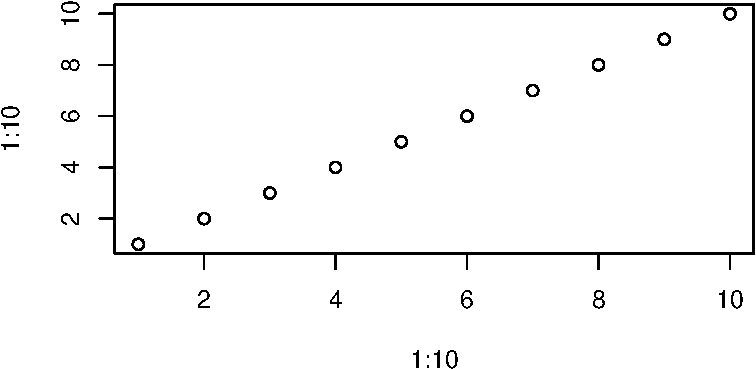
\includegraphics[keepaspectratio]{index_files/figure-pdf/unnamed-chunk-1-1.pdf}}

\textsubscript{Source:
\href{https://Andrapodon.github.io/Master-Thesis-P-kinetics/index.qmd.html}{Article
Notebook}}

\section{Results}\label{results}

\section{Discussion}\label{discussion}

\section{Conclusion}\label{conclusion}

\section{Acknowledgments}\label{acknowledgments}

\section{Legal Disclosure}\label{legal-disclosure}

\section*{References}\label{references}
\addcontentsline{toc}{section}{References}

\phantomsection\label{refs}
\begin{CSLReferences}{1}{0}
\bibitem[\citeproctext]{ref-knuth84}
Knuth, Donald E. 1984. {``Literate Programming.''} \emph{Comput. J.} 27
(2): 97--111. \url{https://doi.org/10.1093/comjnl/27.2.97}.

\end{CSLReferences}

\section{Appendix}\label{appendix}

\section{Supplements}\label{supplements}




\end{document}
